\documentclass[10pt]{article}

\usepackage{spheric}
%%%TITLE
\title{SPH Simulation of Couette Flow with Sinusoidally Moving Solid Boundary}
\date{}

%%AFFILIATIONS
\author[$\relax$]{Haiqiao LI$^\dagger$}
\author[$\relax$]{Hantao LIU}
\author[$\relax$]{Jianzhong CHANG}

\affil[$\relax$]{Laboratory of Energy and Environment and Computational Fluid Dynamics, North University of China, Taiyuan, China}

\affil[$\relax$]{\email{\dagger}{Lihaiqiao8@sina.com}}


%%DOCUMENT
\begin{document}

\maketitle

%\SelectedTopics{}

%%PLEASE PUT YOUR ABSTRACT HERE
\begin{abstract}
The transport of lubricating oil between the cylinder liner and the piston provides a prerequisite for the internal combustion engine normal and long-term operation. Dongfang \cite{bai2012modeling} pointed out that oil transport at the skirt-liner interface can be simplified as two simple models: one is the Couette flow (shear flow) which is driven by the viscous drag force and the inertia acting on the fluid due to the relative movement of the surfaces. The other is the Poiseuille flow (pressure flow), which is driven by the pressure gradient. However, the oil transport between the piston and the piston skirt is closer to the former. In this paper, the motion process of the piston is simplified to the sinusoidal periodic motion. The SPH method \cite{liu2003smoothed} is used to simulate the Couette flow under the sinusoidal period dragged speed for the first time. The velocity distribution of the flow field and the speed variety of different positions are studied under different dynamic viscosity coefficients of oils, different amplitudes of velocity and different frequencies of speed variety. This paper aims to provide a feasible approach to further study the lubrication between the cylinder liner and the piston in the internal combustion engine.

\begin{figure}[!htb]
\begin{minipage}[t]{0.46\linewidth}
\centering
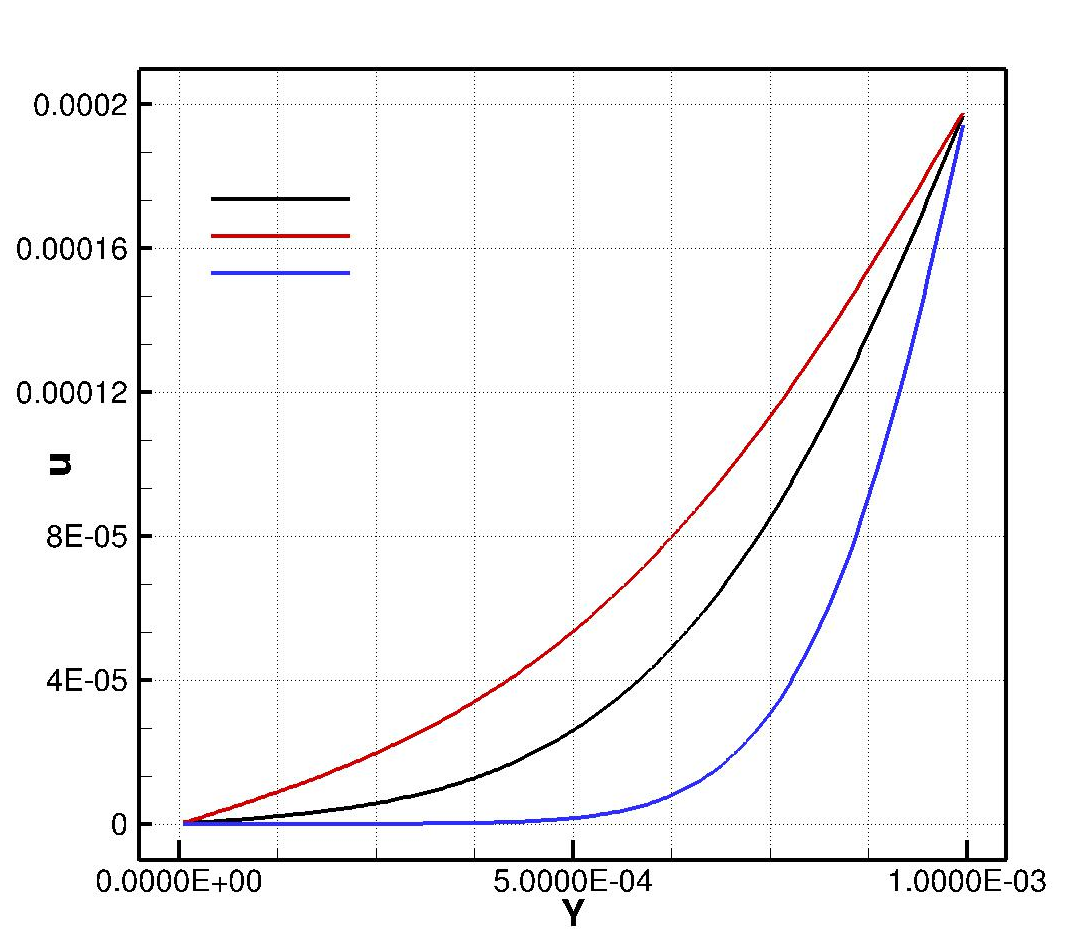
\includegraphics[width=0.8\textwidth]{34-11.png}\\
(a)
\end{minipage}
\begin{minipage}[t]{0.05\linewidth}
~
\end{minipage}
\begin{minipage}[t]{0.46\linewidth}
\centering
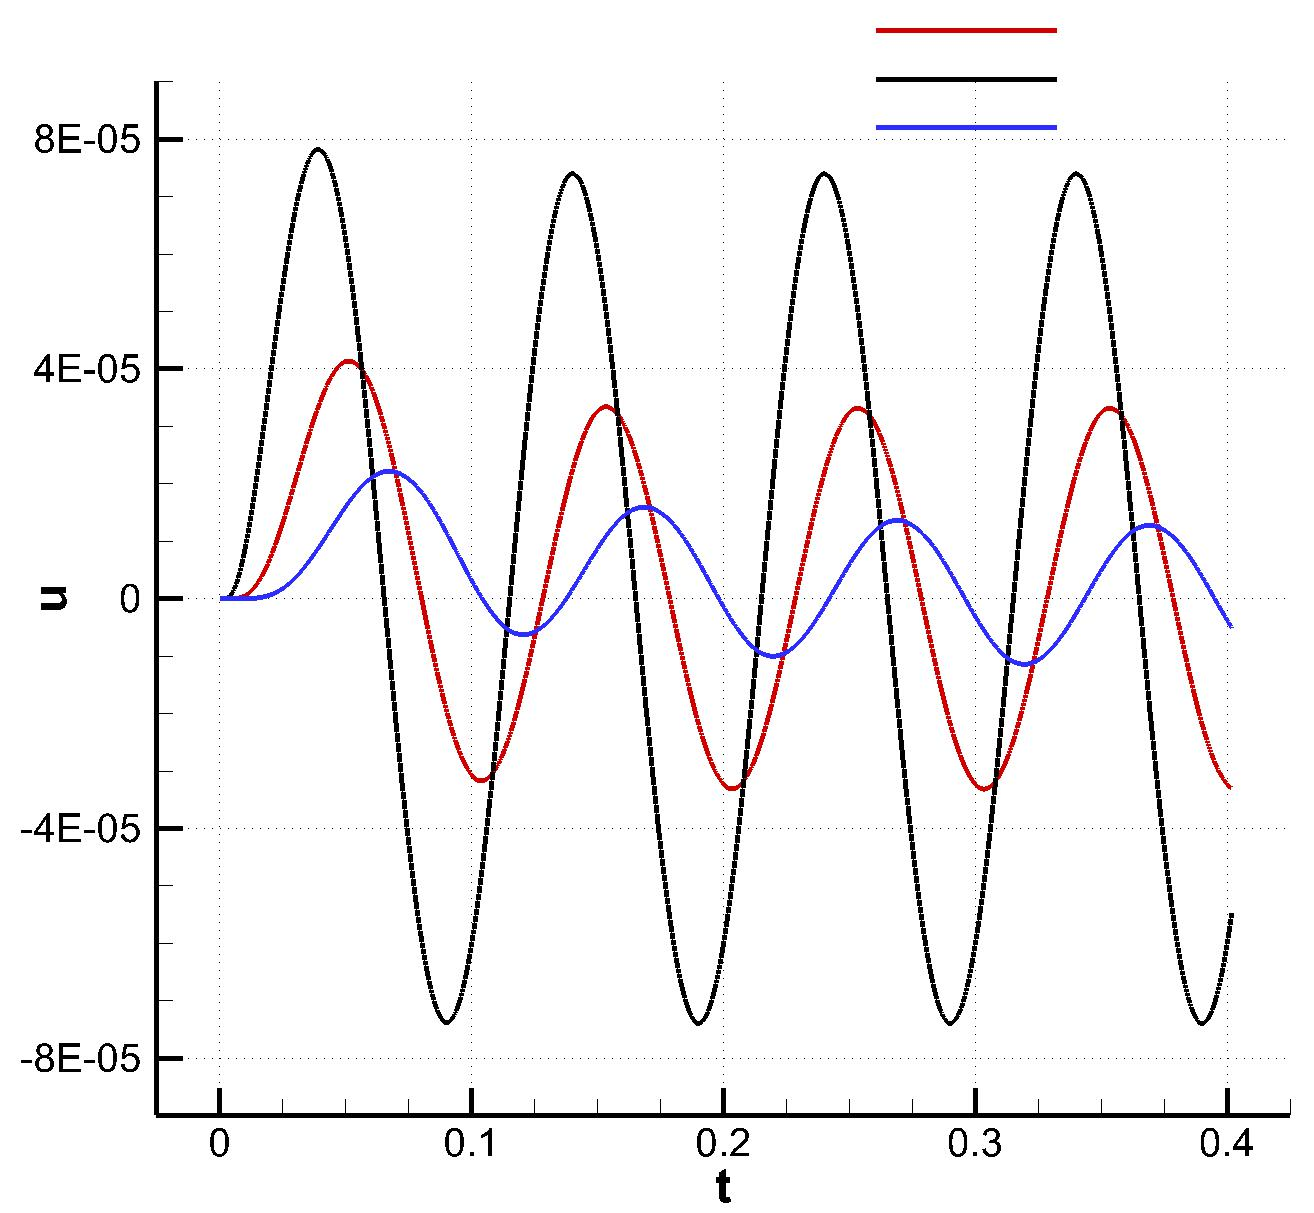
\includegraphics[width=0.8\textwidth]{34-12.png}\\
(b)
\end{minipage}

\begin{minipage}[t]{0.46\linewidth}
\centering
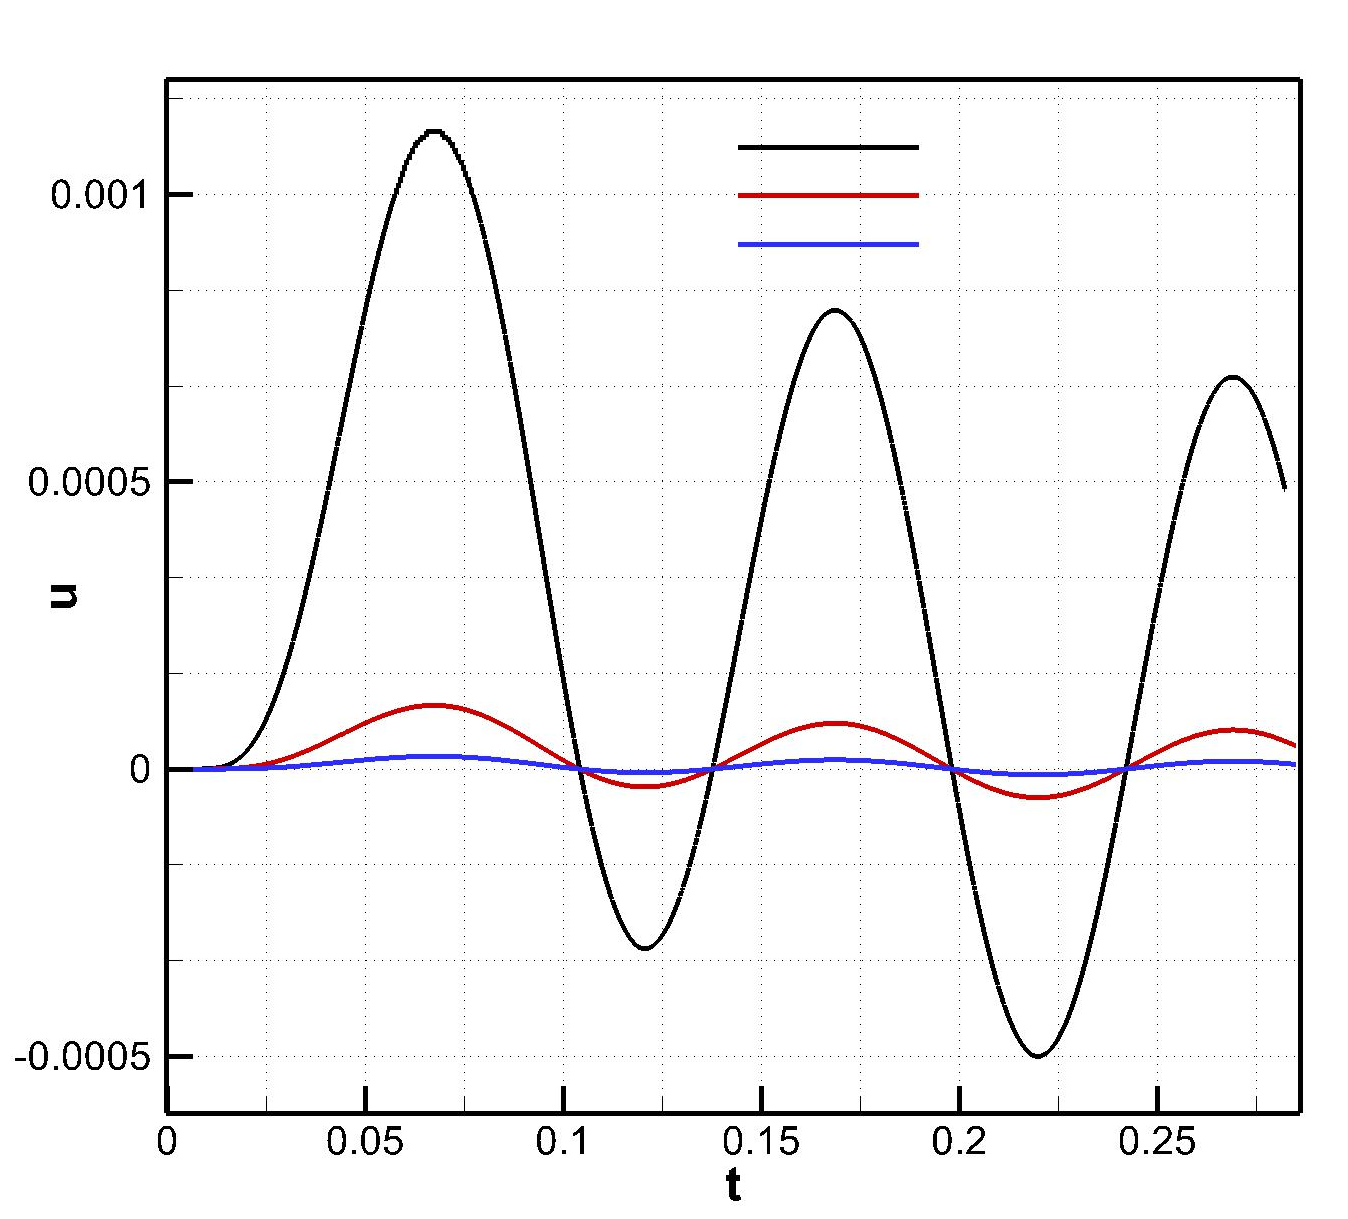
\includegraphics[width=0.8\textwidth]{34-13.png}\\
(c)
\end{minipage}
\begin{minipage}[t]{0.05\linewidth}
~
\end{minipage}
\begin{minipage}[t]{0.46\linewidth}
\centering
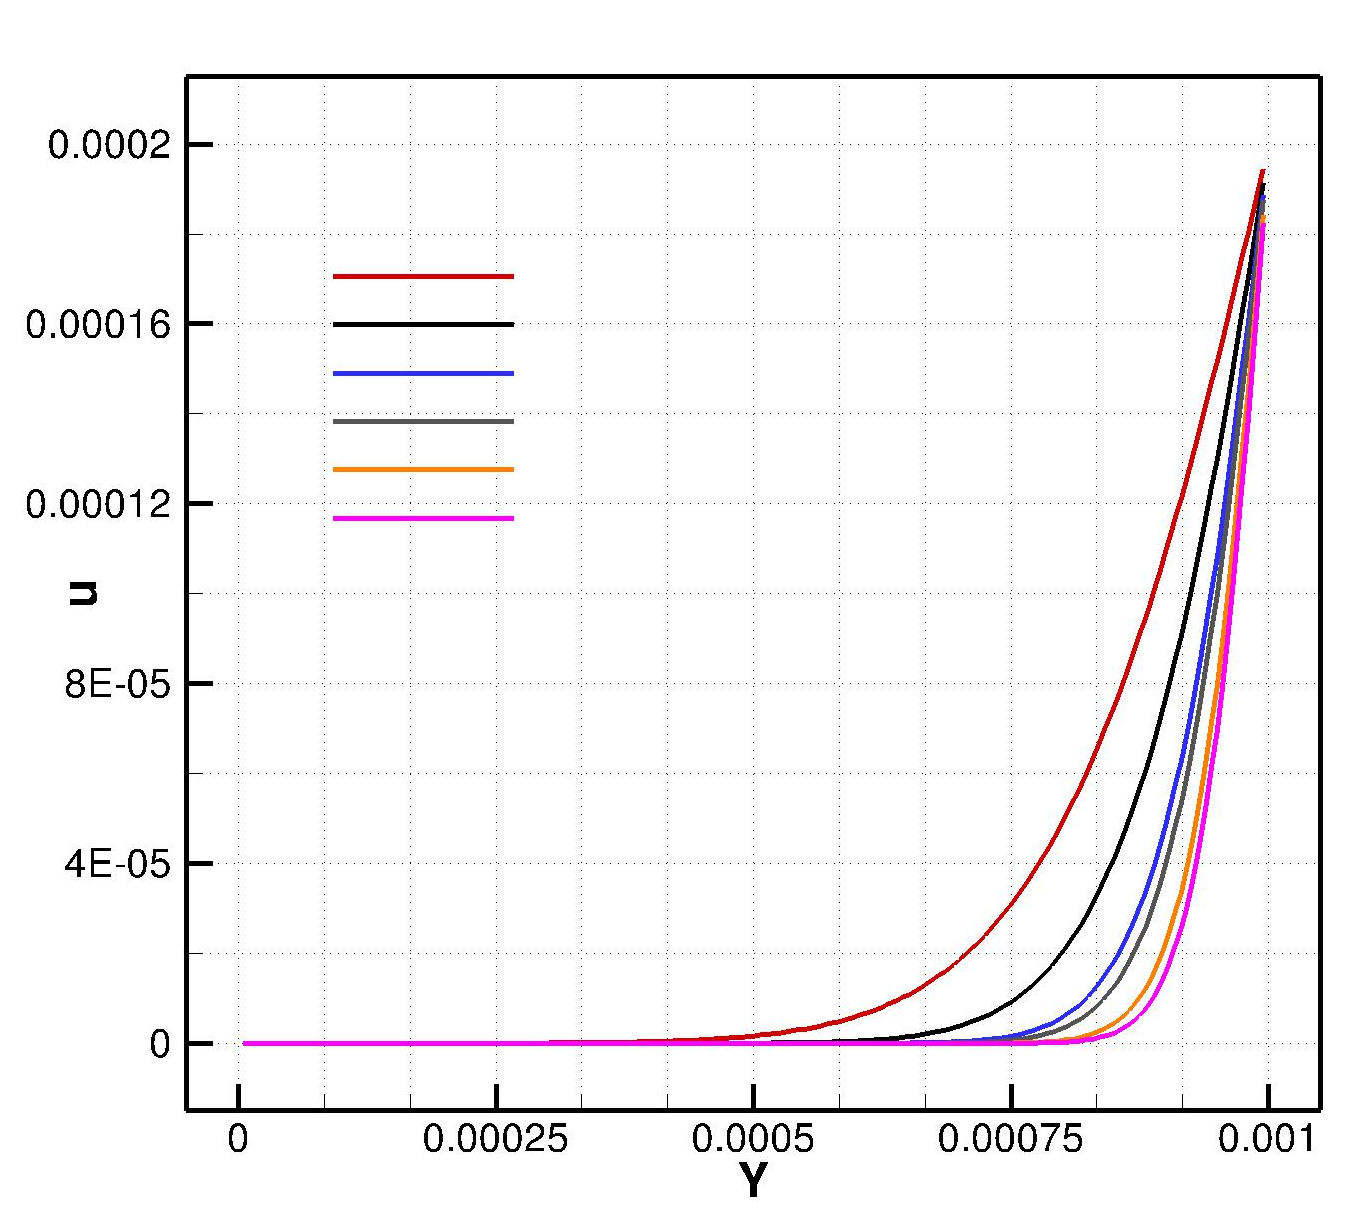
\includegraphics[width=0.8\textwidth]{34-14.png}\\
(d)
\end{minipage}
\caption{The velocity distribution and the speed variety curves. (a. The velocity distribution along the y-direction of calculation area at T/4 under different dynamic viscous coefficients, $u_0=2\times 10^{-4}$ m/s and $f=10$. b. The velocity curve in the $x$ direction over time at $y=5.05\times 10^{-4}$ m under different dynamic viscous coefficients, $u_0=2\times 10^{-4}$ and $f=10$. c. The velocity curve in the $x$ direction over time at $y=5.05\times 10^{-4}$ m under different velocity amplitude, $\mu=1.0\times 10^{-6}~\mathrm{N\cdot s/m^2}$ and $f=10$. d. The velocity distribution along the $y$-direction of calculation area at $T/4$ under different velocity change frequency, $\mu=1.0\times 10^{-6}~\mathrm{N\cdot s/m^2}$ and $u_0=2\times 10^{-4}$ m/s).}\label{fig:}
\end{figure}
In this paper, the boundary drag speed is $u=u_0\sin(2\pi ft)$, where $u_0$ is the amplitude of the velocity, $f$ is the frequency of velocity evolution, $t$ is time, and the period of velocity change is $T$. The calculation area is a rectangular region, which along $x$ is $5\times 10^{-4}$ m and y is $1\times 10^{-3}$ m. The results show that: 1) When the velocity amplitude is small and the velocity change frequency is constant, the viscous drag force plays a leading role in the oil transport process, while the velocity is stabilized after two cycles. 2) When the velocity variation frequency and the dynamic viscosity coefficient keep unchanged, the inertial force become more and more obvious with the increase of the velocity amplitude, while the speed is stable with more cycles. 3) When the speed amplitude and the dynamic viscosity coefficient maintain constant, the inertial force become more and more obvious with the increase of the velocity variation frequency.



\end{abstract}


%%THE END OF ABSTRACT

\addbib

\end{document}
